\chapter{Uso de la librería}\label{chap:libraryUse}
	
	Dada la extensión de la librería, no resulta posible ni deseable mostrar el código fuente completo\footnote{El código completo puede ser consultado y descargado desde la página \url{https://github.com/HugoRedon/Materia}. El apéndice \ref{chap:github} guía al lector en el procedimiento de modificación o extensión del código fuente.}, en este capítulo se presentan pequeños fragmentos de código que muestran la forma de utilizar la librería y su estructura.

	El principal propósito de la biblioteca Materia es realizar el cálculo de propiedades termodinámicas usando ecuaciónes de estado cúbicas. Para cumplir con este propósito distintos modelos se han implementado para realizar el cálculo de los parámetros $a$ y $b$. Este trabajo no pretende explicar los modelos usados, ni su obtención, sin embargo en el apéndice \ref{chap:appendixEquations} se muestran las ecuaciones de algunos de los modelos implementados. 
		
	La clase `Cubic' realiza cálculos de presión, fugacidad, factor de compresibilidad y adimensionamiento de los parámetros $a$ y $b$, pero no calcula los parámetros $a$ y $b$.Para calcular los parámetos $a$ y $b$ existen las clases `Substance' y `Mixture' que definen el cálculo de los parámetros para un compuesto puro o para una mezcla respectivamente. 

	Las clases `Substance' y `Mixture' tienen en común los métodos `calculate\_a\_cubicParameter', `calculate\_b\_cubicParameter', ademas de otros que se condensan en la clase `Homogeneous'.La clase `Homogeneous' utiliza los cálculos de los parámetros de la ecuación cúbica y la clase cúbic para finalmente realizar el cálculo de la fugacidad, presión ,factor compresibilidad, entalpía, entropía y energía libre de Gibbs.

	La clase `Homogeneous' no realiza cálculos de equlibrio, ya que la clase representa una sola fase. Para realizar cálculos de equilibrio existe la clase `Heterogeneous' que contiene dos fases una líquida y una vapor. A través de los cálculos de fugacidad de cada fase y empleando un algoritmo numérico se pueden realizar los cálculos de equilibrio Líquid-Vapor.


	Las secciones del capítulo:
	\begin{itemize}
		\item{Sección} \ref{sec:units} Se definen las unidades que se emplearán durante todo el capítulo.
		\item{Sección} \ref{sec:cubic}  La clase `Cubic' realiza cálculos de presión, fugacidad, factor de compresibilidad y volumen molar.
		\item{Sección} \ref{sec:compounds} La clase `Compound' para definir y utilizar las propiedades del compuesto puro dentro de la librería.
		\item {Sección} \ref{sec:parameters} La clase `Homogeneous' y sus implementaciones `Substance' y `Mixture' para calcular los parámetros de la ecuación cúbica.
		\item {Sección} \ref{sec:homogeneous} La clase `Homogeneous' para realizar cálculos de entalpía, entropía y energía libre de Gibbs.
		\item {Sección} \ref{sec:heterogeneous} La clase `Heterogeneous' y sus implementaciónes `HeterogeneousSubstance' y `HeterogeneousMixutre' para realizar cálculos de equilibrio Líquido-Vapor.
		\item {Sección} \ref{sec:optimization} Las clases `HeterogeneousSubstance' y `HeterogeneousMixture' realizan la optimización de los parámetros de la expresión de alfa en el cálculo del parámetro $a$ de la ecuación cúbica y los parámetros de interacción binaria de las reglas de mezclado para los parámetros de la ecuación de estado cúbica respectivamente.
	\end{itemize}


	% \section{Sistema de Unidades}\label{sec:units}

Las unidades que utiliza la librería se muestran en la tabla \ref{tab:units}.
Durante este escrito se utilizarán las mismas unidades, a menos que se indique lo contrario.


\begin{table}[!h]
	\centering
	\caption{Sistema de unidades empleado por la librería}\label{tab:units}
	\begin{tabular}{ |c| c|c|}
		\hline
			Propiedad & Unidad &\\
		\hline
			Presión & $Pa$ & Pascal\\
			Temperatura & $K$ & Kelvin\\
			Volumen molar & $\frac{m^3}{kg}$ & Metro cúbico sobre kilogramo\\

		\hline
	\end{tabular}
\end{table}%hecho
	% \section{Ecuación de estado cúbica}\label{sec:cubic}

	La ecuación de estado cúbica representada por la clase `Cubic', permite realizar los cálculos de: 
	\begin{itemize}	\itemsep0ex
		\item Presión
		\item Factor de compresibilidad
		\item Volumen molar
		\item Fugacidad
	\end{itemize}

	Cualquier ecuación de estado cúbica se puede crear dentro de la librería \Materia usando los métodos `get' y `set' de la clase `Cubic', ver la sección \ref{subsec:cubicCreation}, pero para comodidad se han definido las ecuaciones de la tabla \ref{tab:cubics} para accederse a través de la clase `EquationsOfState'.

	\begin{table}[!h]
		\centering
		\caption{Ecuaciónes de estado cúbicas accesibles desde la clase `EquationsOfState'}\label{tab:cubics}
		\begin{tabular}{|c |c | c | c | c |}
			\hline
			Ecuación de estado  & $u$ & $w$ & $\Omega_a$&$\Omega_b$\\
			\hline
			Van Der Waals  & $0$ & $0$ & $0,421875$ & $0,125$\\
			\hline
			Peng robinson  & $2$ & $-1$ & $0.45723553$ & $0.077796074$\\
			\hline
			Redlich Kwong  & $1$ & $0$ & $0.42748023$ & $0.08664035$\\
			\hline
			TST  & $2.5$ & $-1.5$ &$ 0.470507$ & $0.0740740$\\
			\hline
		\end{tabular}		
	\end{table}

\subsection{Creación de una ecuación de estado cúbica}\label{subsec:cubicCreation}

	Existen dos formas de crear una ecuación cúbica dentro de la librería \Materia.

	La primera es a través del método contructor, que se accede con la palabra reservada  `new'. De esta manera los valores u y w de la ecuación de estado son iguales a 0 y se les puede asignar un valor diferente haciendo uso de los métods `get' y `set' como se muestra en el código \ref{lst:pengRobinsonCreation}.

	\begin{lstlisting}[label={lst:pengRobinsonCreation},caption=Creación de la ecuación de estado de Peng Robinson usando los metodos `Set' de los parametros u y w]
	Cubic pengRobinson = new Cubic();
	pengRobinson.setU(2);
	pengRobinson.setW(-1);
	pengRobinson.setOmega_a(0.45723553);
	pengRobinson.setOmega_b(0.077796074);
	\end{lstlisting}

	La segunda forma de crear una ecuación de estado es a través de la clase `EquationsOfState'. Para obtener una ecuación con los parámetros previamente establecidos, el fragmento de código \ref{lst:tstCreation} muestra el procedimiento.


	\begin{lstlisting}[label=lst:tstCreation,caption=Creación de la ecuación de estado de TST usando la clase `EquationsOfState']
	Cubic tst = EquationsOfState.twoSimTassone();
	\end{lstlisting}

\subsection{Cálculos con la ecuación cúbica}
	Ya que la clase `Cubic' no realiza los cálculos de sus parámetros estos deben ser proporcionados como argumento de los métodos.

	Los métodos de la clase `Cubic' raramente será necesario usarlos directamente, ya que es dificil obtener el cálculo de los parámetros $a$ y $b$, en cambio la clase `Homogeneous' define el cálculo de los parámetros y de las propiedades que a continuación se muestran.

	\subsubsection{Presión}
	El cálculo en el método `calculatePressure' se realiza según la ecuación \ref{eq:pressure} y se utiliza como se muestra en el código \ref{lst:cubicpressure}.
\begin{lstlisting}[label={lst:cubicpressure},caption={Cálculo de presión con una ecuación de estado cúbica, proporcionando como argumento la temperatura, el volumen y los parámetros $a$,$b$}]
	 double pressure =  cubic.calculatePressure(temperature, volume, a, b);
\end{lstlisting}
	\subsubsection{Factor de compresibilidad}

	Es necesario realizar la solución de la ecuación de estado cúbica, como se muestra en el apéndice \ref{sec:cubicsolution}, para conocer el factor de compresibilidad. La solución de la ecuación se realiza en el método `calculateCompresibilityFactor'.

	El método recibe los parámetros adimensionales A, B y la fase a la cual se desea calcular el factor de compresibilidad. La clase ``Cubic'' tiene los métodos necesarios para transformar los parámetros a y b a su forma adimensional A y B según las ecuaciones \ref{eq:AB}.

	El código \ref{lst:cubiccompresibility} muestra como usar el método.
\begin{lstlisting}[label={lst:cubiccompresibility},caption={Cálculo del factor de compresibilidad con una ecuación de estado cúbica, proporcionando como argumento los parámetros adimensionales $A$,$B$, y la fase a la cual se desea calcular el factor}]
	double z = cubic.calculateCompresibilityFactor(A,B,phase);
\end{lstlisting}
	\subsubsection{Volumen molar}

	La ecuación \ref{eq:volume} proporciona un método para calcular el volume molar a partir del factor de compresibilidad. El código \ref{lst:cubicvolume} muestra el método.
\begin{lstlisting}[label={lst:cubicvolume},caption={Cálculo del volumen molar usando una ecuación de estado cúbica, el método recibe los parámetros de temperatura, presión y factor acéntrico}]
	double volume = calculateVolume(temperature, pressure, z);
\end{lstlisting}	
	\subsubsection{Fugacidad}
	La fugacidad se calcúla segun la ecuación \ref{eq:fugacity}.Para realizar el cálculo de la fugaciad es necesario conocer las derivadas de los parámetros con respecto a la cantidad de moles del componente i, es decir al componente para el cúal se desea realizar el cálculo de fugacidad. El cálculo de la derivada de los parámetros se realiza en las clases que hereden a `Homogeneous', por ejemplo las clases `Substance' y `Mixture'.
	El método se usa como se indica en el código \ref{lst:fugacity}.
\begin{lstlisting}[label={lst:fugacity},caption={Cálculo de fugacidad usando una ecuación de estad cúbica, el método recibe los parámetros de temperatura, presión ,los parámetros de la ecuación cúbica $a$ y $b$, las derivadas con respecto a la cantidad de moles $partial_a$, $partial_b$ y finalmente la fase a la que se desea el cálculo de la fugacidad.}]
	double fugacity = calculateFugacity(temperature, pressure,
										 a, b, parcial_a, parcial_b,phase);
\end{lstlisting}


%hecho
	% \section{Compuestos}\label{sec:compounds}

La clase `Compound' permite definir las propiedades de un compuesto puro y utilizarlas dentro de la librería \Materia.

Propiedades como la temperatura crítica, presión crítica, factor acéntrico y los parámetros para las expresiones de \alfa pueden obtenerse de esta clase como se muestra en el código \ref{lst:compounds}.

\begin{lstlisting}[caption={Se muestra la creación de un objeto tipo `Compound' para definir y utilizar las propiedades del cyclohexano, haciendo uso de los métodos `get' y `set'.},label={lst:compounds}]
Compound compound = new Compound("Cyclohexane");
compound.setCriticalPressure(4073000);
compound.setCriticalTemperature(553.5);
compound.setAcentricFactor(0.211);
....
double acentricFactor = compound.getAcentricFactor();
double pc = compound.getCriticalPressure();
double tc = compound.getCriticalTemperature();
\end{lstlisting}






%hecho
	% \section{Parámetros de la ecuación de estado cúbica}\label{sec:parameters}

El cálculo de los parámetros depende de la cantidad de compuestos presentes en el sistema.

\begin{itemize}
 \item Para los compuestos puros la clase `Substance' define el cálculo de los parámetros usando una expresión de $\alpha$ , los parámetros $\Omega_a$ y $\Omega_b$ de la ecuación de estado y las propiedades del compuesto puro.
 \item Para las mezclas, la clase `Mixture' define el cálculo de los parámetros usando una regla de mezclado y el cojunto de los parámetros  $a$ y $b$ calculados a partir de los compuestos puros.
\end{itemize}


Esta estructura se muestra en laf figura \ref{fig:homogeneousCalculations}

\begin{figure}[!h]
  
  \centering
    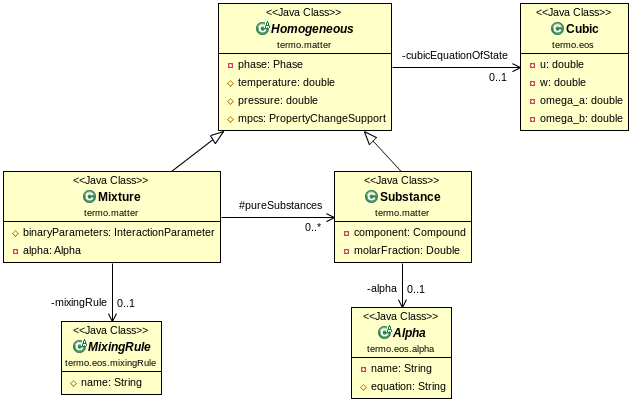
\includegraphics[scale=0.7]{homogeneousCalculations.png}
    \caption{Estructura de la librería para el cálculo de propiedades.}
    \label{fig:homogeneousCalculations}
\end{figure}

Nótese de la figura \ref{fig:homogeneousCalculations} los siguiente:
\begin{itemize}
	\item Que la clase `Homogeneous' contiene una ecuación del tipo `Cubic'.
 	\item Que las clases `Substance' y `Mixture' heredan las propiedades de la clase `Homogenous', como la ecuación cúbica, y puede hacer uso de ella.

\end{itemize}

	Cualquiera de las dos implementaciones de la clase `Homogeneous' tiene los métodos necesarios para calcular los parámetros de la ecuación cúbica según el código \ref{lst:homogeneousParameters}.

\begin{lstlisting}[caption=Cualquier objeto tipo `Homogeneous' puede calcular los parámetros de la ecuación de estado cúbica a y b, label={lst:homogeneousParameters}]
	Homogeneous homogeneous = ...// Objeto tipo `Homogeneous'.
	double a = homogeneous.calculate_a_cubicParameter();
	double b = homogeneous.calculate_b_cubicParameter();
\end{lstlisting}


\subsection{Compuesto puro}\label{subsec:substance}

Como se muestra en la figura \ref{fig:homogeneousCalculations} la clase `Substance' continene una expresión de $\alpha$, y una ecuación de estado, necesarias para realizar el cáculo de los parámetros, segun las ecuaciones \ref{eq:a} y \ref{eq:b}. 

La expresión de $\alpha$ puede ser una función de la temperatura, las expresiones implementadas en el presente trabajo se muestran en la tabla \ref{tab:alphas}.

\begin{table}[!h]
	\centering
	\caption{Expresiónes de $\alpha$ disponibles en la librería}\label{tab:alphas}
	\begin{tabular}{|c|c|c| }
		\hline
		Expresión & Parámetros & Ecuación de estado\\
		\hline
		Soave    &  ---& PR\\
		Peng and Robinson & ---& PR \\
		Mathias & $A$ & SRK\\
		Stryjek and Vera & $k_1$ & PRSV\\
		Adachi and Lu & $A,B$&SRK,PR\\
		Soave & $A,B$&SRK,PR\\
		Melhem, et al. & $A,B$&SRK,PR\\
		Androulakis et al. & $A,B,C$& SRK,PR\\
		Mathias and Copeman & $A,B,C$& SRK,PR\\
		Yu and Lu & $A,B,C$&SRK,PR\\
		Stryjek and Vera & $A,B,C$&PR\\
		Twu & $L,M,N$&TST\\
		Twu & ---&TST,PR\\
		GCEOS & ---& (Cualquier u y w)\\
		\hline
	\end{tabular}
\end{table}
\subsubsection{Creación de un objeto tipo `Substance'}\label{subsub:substanceCreation}

Es necesario utilizar el método constructor de la clase `Substance' para crear un objeto de este tipo, se debe proporcionar como parámetros la ecuación de estado deseada, la exprsión de $\alpha$, una instancia de la clase `Compound' como se muestra en la sección \ref{sec:compounds} y la fase de la substancia.

En la sección \ref{subsec:cubicCreation} se mostró como crear una ecuación de estado cúbica previamente definida, a través de la clase `EquatiosOfState'. Los valore de $\Omega_a$ y $\Omega_b$ se muestran en la tabla \ref{tab:cubics}. De forma muy similar al de las ecuaciońes de estado,la selección de la expresión de $\alpha$ se realiza a través de la clase `Alphas'.

El código \ref{lst:substanceCreation} muestra como crear una objeto del tipo substancia.

\begin{lstlisting}[caption={Creación de un objeto tipo `Substance' para el compuesto Ciclohexano, con la ecuación de estado Soave Redlich Kwong y la expresión de $\alpha$ de mathias },label={lst:substanceCreation}]

Compound compound = new Compound("Cyclohexane");
compound.setCriticalPressure(4073000);
compound.setCriticalTemperature(553.5);
compound.setAcentricFactor(0.211);


Cubic srk = EquationsOfState.redlichKwongSoave();
Alpha mathias = Alphas.getMathiasExpression();


Substance substance = new Substance(srk,mathias, compound,Phase.LIQUID);
\end{lstlisting}

	Finalmente se utiliza el objeto creado para realizar el cálculo de los parámetros de la ecuación de estado cúbica, en el código \ref{lst:substanceParams}.

\begin{lstlisting}[caption={Cálculo de los parámetros para la ecuación de estado cúbica con la clase `Substance'.},label={lst:substanceParams}]
double a = substance.calculate_a_cubicParameter();
double b = substance.calculate_b_cubicParameter();
\end{lstlisting}
 

Nótese que el código \ref{lst:homogeneousParameters} y el código \ref{lst:substanceParams} es idéntico y aunque parece redundate, solo se muestra para señalar el polimorfismo de la librería , es decir que el objeto substance es del tipo `Homogeneous' además del tipo `Substance', y tiene accesso a los métodos en las dos clases.


\subsubsection{Mezcla}\label{subsec:mixture}

El cálculo de los parámetros para una mezcla depende de la regla de mezclado, y en el caso de las reglas de mezclado basadas en la energía libre de exceso, también del modelo de actividad.

Las reglas de mezclado incluidas en este trabajo se muestran en la tabla \ref{tab:mixingrules}, y los modelos de actividad se listan en la tabla \ref{tab:activitymodels}.

\begin{table}[!h]
	\caption{Reglas de mezclado implementadas}\label{tab:mixingrules}
	\begin{tabularx}{\textwidth}{|X|X|X|}
		\hline
		Regla & Parámetros & \\
		\hline
		Van Der Waals & $k_{ij}$ & $k_{ij} = k_{ji}$ \\
		Mathias-Klotz-Prausnitz& $k_{ij}$ & $k_{ij} \neq k_{ji}$ \\
		Huron Vidal & Según el model de actividad & \\
		Wong Sandler & $k_{ij}$ + los parámetros del modelo de actividad & $k_{ij} = k_{ji}$ \\
		\hline
	\end{tabularx}
\end{table}

\begin{table}[!h]
	\caption{Modelos de actividad }\label{tab:activitymodels}
	\begin{tabularx}{\textwidth}{|X|X|X|}
		\hline
		Modelo de actividad & Parámetros & \\
		\hline
		Wilson & $a_{ij}$, $b_{ij}$  & \\
		NRTL & $a_{ij}$, $b_{ij}$, $\alpha_{ij}$ & $\alpha_{ij} = \alpha_{ji}$ \\
		\hline
	\end{tabularx}
\end{table}
\subsubsection{Creación de un objeto tipo `Mixture'}\label{subsub:mixtureCreation}

Un objeto tipo `Mixture' contiene dentro de sí un conjuto de objetos tipo `Substance', esto hace que su creación sea mas compleja. Se ha escrito la clase `MixtureBuilder' para facilitar la creación de los objetos de la clase `Mixture'.

La clase `MixtureBuilder' facilita la creación de los objetos `Substance' que forman el conjunto de compuestos de la mezcla, y permite asignar una expresión de $\alpha$ diferente para cada compuesto.

El código \ref{lst:mixturecreation} muestra la creación de una mezcla, donde la expresión de $\alpha$ es la misma para cada compuesto puro. 

\begin{lstlisting}[caption={Creación de una mezcla con la clase `MixtureBuilder' asignando la misma expresión de $\alpha$ para cada compuesto puro.}, label={lst:mixturecreation} ]

Compound cyclohexane = new Compound("Cyclohexane");
cyclohexane.setCriticalPressure(4073000);
cyclohexane.setCriticalTemperature(553.5);
cyclohexane.setAcentricFactor(0.211);

Compound pentane = new Compound("N-pentane");
pentane.setCriticalPressure(3370000);
pentane.setCriticalTemperature(469.7);
pentane.setAcentricFactor(0.251);

Cubic equationOfState = EquationsOfState.pengRobinson();
Alpha alpha = Alphas.getMathiasAndCopemanExpression();

Mixture mixture = new MixtureBuilder()
			.addCompounds(cyclohexane,pentane)
			.setAlpha(alpha)
			.setEquationOfState(equationOfState)
			.setPhase(Phase.VAPOR)
			.build();

\end{lstlisting}

Es posible crear la mezcla con una expresión de $\alpha$ diferente para cada compuesto puro según el código \ref{lst:mixtureParametersDifAlphas}. 


\begin{lstlisting}[caption={Código para el cálculo de los parámetros de la ecuación de estado en una mezcla, con diferentes expresiones de $\alpha$},label={lst:mixtureParametersDifAlphas}]
Mixture mixture = new MixtureBuilder()
			.addCompound(cyclohexane,Alphas.getPengAndRobinsonExpression())
			.addCompound(pentane,Alphas.getStryjekAndVeraExpression())
			.setEquationOfState(eos)
			.setPhase(phase)
			.setMixingRule(mixingRule)
			.setInteractionParameter(k)
			.build();
\end{lstlisting}

Finalmente se pueden calcular los parámetros de la ecuación cúbica con el código \ref{lst:mixtureParameters}.

\begin{lstlisting}[caption={Cálculo de parámetros de la mezcla},label={lst:mixtureParameters}]
double a = mixture.calculate_a_cubicParameter();
double b = mixture.calculate_b_cubicParameter();
\end{lstlisting}
%hecho
	% \section{Ecuación de capacidad calorífica}\label{sec:cp}

	Los cálculos de entalpía y entropía necesitan de una ecuación de capacidad calorífica.

	La librería \Materia  define una interface para obligar que todas las implementaciones de la ecuación tengan los métodos para calcular la entalpía y entropía del gas ideal según la ecuaciones \ref{eq:idealgasenthalpy}, \ref{eq:idealgasentropy}.

	Incluidas para el presente trabajo la librería \Materia implementa las ecuaciones 107 del DIPPR y una ecuación Polinomial obtenida de la base de datos Chemsep ver ecuaciones \ref{eq:dippr107} y \ref{eq:chempse16}.
	
	Predeterminadamente se usa la ecuación 107 de DIPPR.
	% \section{Materia homogénea}\label{sec:homogeneous}

	La clase `Homogeneous' representa a las substancias o mezclas que se encuentran en una sola fase, las propiedades que se pueden calcular de una fase son: 
\begin{itemize}
	\item fugacidad
	\item presión
	\item factor compresibilidad 
	\item volume molar
	\item entalpía 
	\item entropía 
	\item energía libre de gibbs.
\end%hecho			
	% \section{Equilibrio Líquido-Vapor}\label{sec:heterogeneous}

	La clase `Heterogeneous' se encarga de los cálculos de equilibrio entre las fases líquido y vapor. La clase contiene dos instancias de la clase `Homogeneous' que representan a la clase líquida y a la clase vapor. La clase implementa los algoritmos numéricos para igualar los cálculos de la fugacidad entre las fases.

	Los cálculos de equilibrio que se implementan en este trabajo son:

	\begin{itemize}

		\item Substancias
			\begin{itemize}
				\item Temperatura de saturación.
				\item Presión de saturación.
			\end{itemize}

		\item Mezclas
	\begin{itemize}
		\item Presión de burbuja, sección \ref{subsec:bubblepressure}.
		\item Presión de rocío, sección \ref{subsec:dewpressure}.
		\item Temperatura de burbuja, sección \ref{subsec:bubbletemperature}.
		\item Temperatura de rocío, sección \ref{subsec:dewtemperature}.
		\item Flash temperatura-presión \ref{subsec:flash}.
	\end{itemize}

	\end{itemize}

	Los algoritmos son muy similares, las principales diferencias consisten en la función objetivo.

	La clase `HeterogeneousSubstance' realiza los cálculos de equilibrio para las substancias y la clase `HeterogeneousSubstance' realiza los cálculos de equilibrio para las mezclas, en la figura \ref{fig:heterogeneous} ser muestra la estructura.

\begin{figure}[!h]
  \centering
    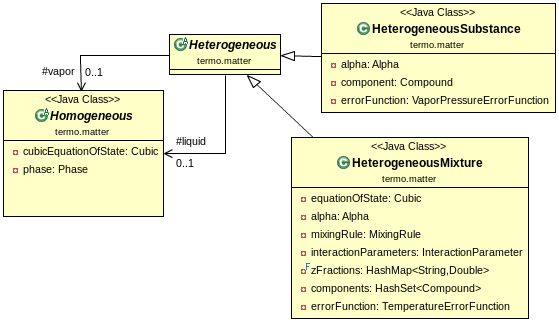
\includegraphics[scale=0.7]{heterogeneous.png}
    \caption{Estructura de la librería para el cálculo de equilibrio Líquido-Vapor.}
    \label{fig:heterogeneous}
\end{figure}

	Los cálculos de la presente sección se realizan de forma muy similar, primero indicando la variable conocida con el método `set', después invocando el método que realiza el algoritmo para conocer la incognita, el método puede recibir o no un estimado inicial y finalmente obtener el resultado de la variable con el método `get'.

	Cada sección muestra el uso de la librería con fragmentos de código que realizan el cálculo con y sin el estimado inicial. También se indica que método se usa para estimar la varible incognita en caso de no proporcionar un estimado inicial.

		
%hecho			
	% \section{Estimación de parámetros}\label{sec:optimization}

	Para el cálculo del parámetro $a$ de la ecuación de estado cúbica es necesaria una expresión de $\alpha$ como se muestra en la ecuación \ref{eq:a}. Todas las expresiones de $\alpha$ escritas para este trabajo se listan en la tabla \ref{tab:alphas}. Estas expresiones pueden tener parámetros que deben ser estimados en base a datos experimentales de compuestos puros. La estimación de los parámetros de $\alpha$ se realiza en la clase `HeterogeneousSubstance'.

	Para realizar el cálculo de los parámetros de le ecuación cúbica para una mezcla, es necesario utilizar una regla de mezclado como se mostró en la sección \ref{subsec:mixture}. Las reglas de mezclado escritas para este trabajo se listan en la tabla \ref{tab:mixingrules}. Las reglas de mezclado usan parámetros que deben ser estimados en base a datos experimentales de mezclas binarias. La estimación de los parámetros binarios se realiza en la clase `HeterogeneousMixture'.

	\begin{itemize}
		\item{Sección} \ref{subsec:alphaoptim} Estimación de parámetros de la expresión de $\alpha$.
		\item{Sección} \ref{subsec:binaryoptim} Estimación de parámetros de interacción binaria para las reglas de mezclado.
	\end{itemize}

	





%hecho
				